\documentclass[11pt]{hyu_thesis}

\begin{document}

\abovedisplayskip=16pt
\abovedisplayshortskip=11pt
\belowdisplayskip=16pt
\belowdisplayshortskip=11pt
	
\frontmatter

\tableofcontents
\newpage
\listoffigures
\newpage
\listoftables
\newpage

\mainmatter

\section*{ABSTRACT}
\addcontentsline{toc}{section}{ABSTRACT}
Video synopsis allows us to analyze security videos efficiently by condensing or shortening a long video into a short one. To generate a condensed video, moving objects (a.k.a. object tubes) in the video are rearranged in the temporal domain using a predefined objective function. The objective function consists of several energy terms which play important roles in making a visually appealing condensed video. One of the energy terms, collision energy, creates a bottleneck in the computation because it requires two object tubes to calculate the degree of collision between them. Existing approaches try to reduce the computation time of the collision energy calculation by reducing the number of tubes processed at once. However, those approaches are not sufficient to generate condensed video when the number of object tubes becomes large.

In this letter, we propose a fast Fourier transform (FFT)-based parallelized tube rearrangement algorithm. To take advantage of both parallel processing and FFT, we represent object tubes as 3D binary matrices (occupation matrices). An objective function of the tube rearrangement problem is defined on the occupation matrix, and a starting position for each tube in the temporal domain is then determined by optimizing the objective function. Throughout the experiments, the proposed algorithm took a much shorter time to condense the video than existing algorithms, while other performance metrics were similar.
\newpage

\section{Introduction}
\label{sec:intro}
\subsection{Motivation}
\label{sec:intro:motivation}
The field of security video summarization has been studied for decades to reduce burdens of browsing large amount of video footages. Earlier approaches~\cite{Smith1998,Petrovic2005,Hoferlin2011} prior to video synopsis~\cite{Rav-Acha2006,Pritch2007,Pritch2008} suffered from several disadvantages including low frame condensation ratio (FR) or missing information, when the frame length of the input video was long. Fundamental building blocks of such approaches were image frames, which means that they tried to select a subset of image frames representing the original video best. On the other hand, building blocks of video synopsis~\cite{Rav-Acha2006,Pritch2007,Pritch2008} are moving objects extracted from the scene, called \textit{object tubes}. In the video synopsis framework, the object tubes are rearranged in the temporal domain and stitched back with background images to generate a short and condensed video. This difference allows video synopsis to efficiently utilize the spatial domain of the video and to drastically improve the FR as compared to the earlier approaches.

Among the diverse research topics in video synopsis, solving the optimization problem for determining starting positions (starting labels) of the object tubes in the temporal domain greatly affects the system performance regarding computation time. This problem is simply denoted as \textit{a tube rearrangement problem}.

In the pioneering work of video synopsis by Pritch~\etal~\cite{Pritch2008}, the tube rearrangement problem is formulated as Markov Random Fields (MRFs)~\cite{Kolmogorov2004} with four energy terms: activity, collision, temporal consistency, and background consistency. The starting label for each object tube is then determined by minimizing the energy function of MRFs with a simulated annealing~\cite{Kirkpatrick1983} or greedy optimization algorithm~\cite{Cormen2009}. During the optimization process, calculating pairwise energy terms (in this case, collision and temporal consistency) becomes a bottleneck for computation speed, because such calculation has $O(TK^2)$ complexity, where $T$ is the number of time steps and $K$ is the total number of object tubes.

In order to cope with the problem, Pritch~\etal~\cite{Pritch2009} suggest
a clustering based optimization algorithm. It divides object tubes into several subsets; then, the optimization algorithm is conducted on each subset. Since the number of object tubes belonging to each subset is much smaller than $K$, execution time of the optimization algorithm is greatly reduced. However, its condensation result depends on the performance of the clustering algorithm which has a chance to
generate inappropriate clusters.

An alternative approach to tube rearrangement is an online video synopsis~\cite{Huang2014,ShikunFeng2012,JianqingZhu2015,He2017,Fu2014}, which solves a stepwise optimization problem. In stepwise optimization, instead of considering entire object tubes at the same time, the starting labels of the object tubes are determined one by one. Therefore, it requires less computational power and memory space than batch or offline video synopsis. In addition, since online video synopsis optimizes the object tubes in chronological order, it is inessential to consider temporal and background consistencies. Therefore, the most of online video synopsis frameworks mainly consider the collision energy during the optimization.

Based on such advantages, recent studies of online video synopsis focused on finding efficient ways of solving a stepwise optimization problem: for example, the maximum a posteriori estimation~\cite{Huang2014}, a Tetris-like tube rearrangement strategy~\cite{ShikunFeng2012,JianqingZhu2015}, and a potential collision graph~\cite{He2017}. 
Even though these existing algorithms have their own virtue, they have lack of considerations of multi-core environment, which means that there are still rooms for improvements.

In this dissertation, the tube rearrangement problem is reformulated as a suitable form for parallel processing, and the novel concurrent optimization algorithm based on 1D convolutions is proposed to accelerate the optimization process. As in other online tube rearrangement algorithms~\cite{Huang2014,ShikunFeng2012,JianqingZhu2015,He2017,Fu2014}, the collision energy is primarily considered during the tube rearrangement. As a preprocessing step, the proposed algorithm reshapes object tubes into probabilistic occupation matrices of $\mathcal{M} \times \mathcal{N} \times \mathcal{T}$ dimension, where $\mathcal{M}$ and $\mathcal{N}$ represent the spatial domain, and $\mathcal{T}$ represents the time domain. This occupation matrix becomes a fundamental building block of the proposed algorithm. Then, the collision energy between two object tubes can be computed as element-wise multiplications of two occupation matrices. This process can be accelerated by utilizing Fast Fourier transform (FFT)~\cite{Oppenheim2009} in conjunction with parallel computing; therefore, the proposed algorithm can effectively determine the starting labels of numerous object tubes in very short amount of time.

\subsection{Related works}
\label{sec:intro:related}
A summary of the recent advances in video synopsis is presented as follows. Nie~\etal~\cite{Nie2014} rearrange object tubes in both temporal and spatial domain to generate more condensed videos. Zhu~\etal~\cite{Zhu2014} and Mahapatra~\etal~\cite{Mahapatra2016} extend the concept of video synopsis to the multi-camera network. Wang~\etal~\cite{Wang2013} and Zhong~\etal~\cite{RuiZhong2014} utilize the compressed domain to generate synopsis videos efficiently. X. Li~\etal~\cite{Li2016a} scale down object sizes to reduce collisions in the synopsis video. Z. Li~\etal~\cite{ZhuangLi2009} and K. Li~\etal~\cite{Li2016} introduce a seam carving method to remove redundant information from the original video.

\subsection{Dissertation overview}
\label{sec:intro:overview}
The rest of the dissertation is organized as follows. Section \ref{sec:basic_form} introduces the basic formulation of video synopsis and details of the proposed tube rearrangement algorithm are described in Section \ref{sec:proposed}. Section \ref{sec:framework} contains explanations of other components that the online video synopsis consists of. Section \ref{sec:exp} presents experimental results, and the dissertation is concluded in Section \ref{sec:conc}.

\section{Basic formulation of video synopsis}
\label{sec:basic_form}

In this section, the basic formulation of video synopsis introduced in the pioneering works~\cite{Rav-Acha2006,Pritch2007,Pritch2008} is described to show which part of the formulation has to be changed for parallel processing. In addition, the reason why online video synopsis mainly considers collision energy is explained in detail.

As in Fig.~\ref{fig:video_synopsis}, a principal objective of video synopsis is shortening length of the input video by relocating object tubes in temporal domain. In other words, we try to find the best combination of object tubes' starting positions in temporal domain (starting labels). In the field of video surveillance, a definition of the best combination can be different from specific applications. However, based on the paper of Pritch~\etal~\cite{Pritch2008}, the condensed video with the best starting label combination should have following characteristics.
\begin{itemize}
\item Objects of interests should be appeared in the condensed video.
\item Rearranged object tubes should seamlessly rendered in the condensed video.
\item The condensed video has significantly shorter length than the input video.
\item Dynamics of objects or interactions between the objects should be understood in the condensed video.
\end{itemize}
To achieve the characteristics, the batch video synopsis~\cite{Pritch2008} utilizes four energy terms as described in Section~\ref{sec:intro}: activity, background consistency, collision, and temporal consistency. The order of the energy terms are matched with that of the characteristics.

\begin{figure}
\begin{center}
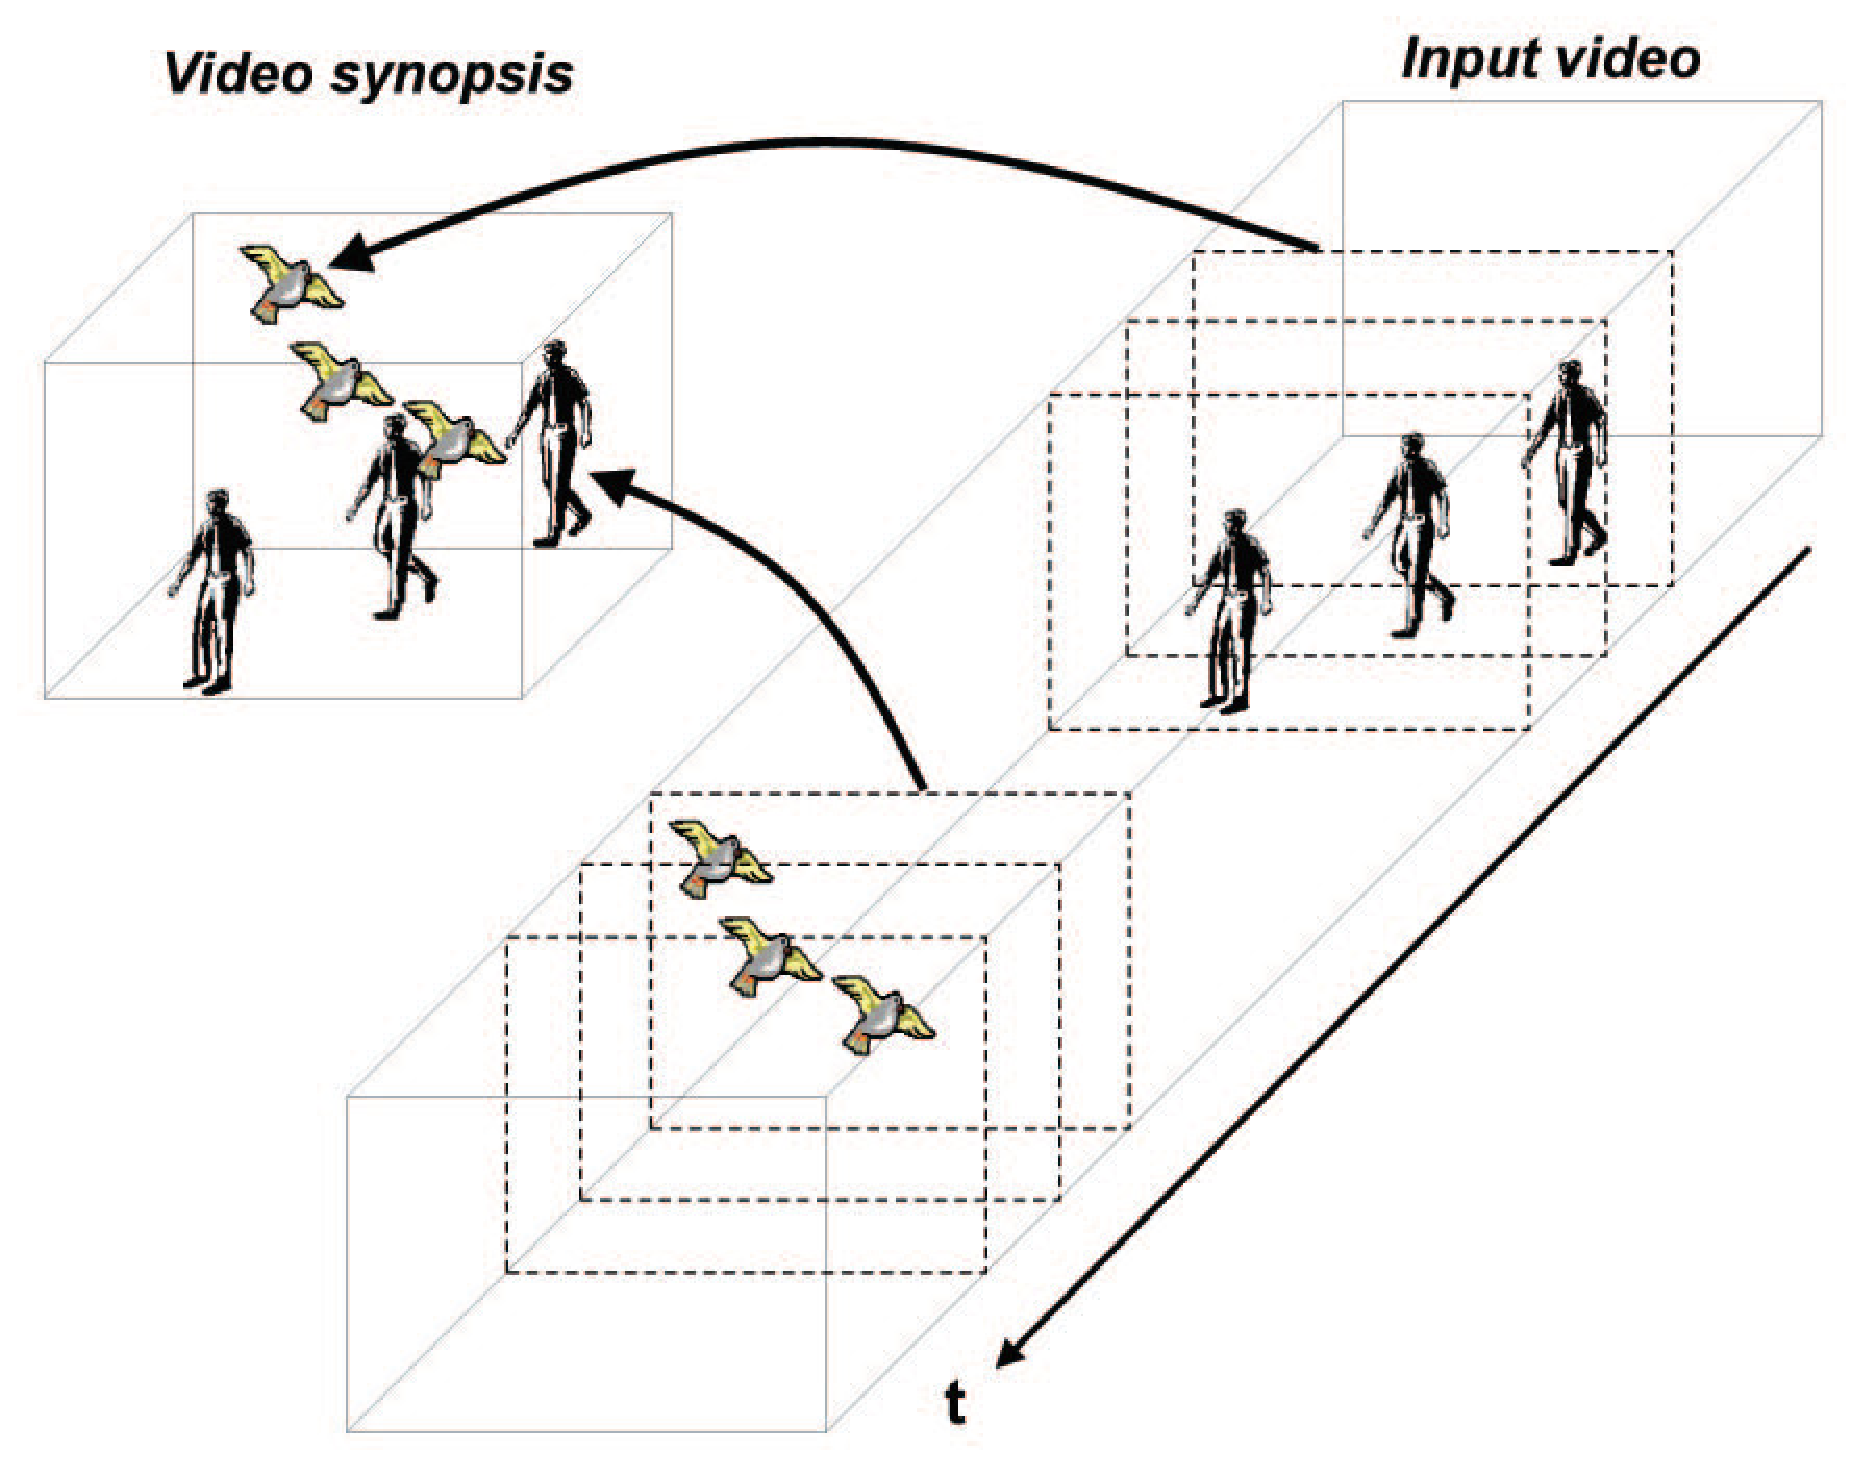
\includegraphics[width=\linewidth]{video_synopsis.eps}
\end{center}
\caption{A concept diagram of video synopsis~\cite{Pritch2009}. The bird and man appeared at different time in the original video are rearranged in temporal domain, and then displayed simultaneously in the condensed video.}
\label{fig:video_synopsis}
\end{figure}

Assume that $L=\{l_0,...,l_N\}$ is a set of starting labels for $N$ object tubes; then, an objective function $E(L)$ can be defined as
\begin{equation}
\label{eq:basic_form}
E(L)=\sum_{l_i \in L} \left( E_a(l_i) + \gamma E_s(l_i) \right) + \sum_{l_i,l_j \in L} \left( \alpha E_t(l_i, l_j) + \beta E_c(l_i, l_j) \right),
\end{equation}
where $E_a$, $E_s$, $E_t$, and $E_c$ are activity, background consistency, temporal consistency, and collision energies, respectively. In addition, $\alpha$, $\beta$, and $\gamma$ are weight parameters for controlling importance between the energies.

\subsection{Activity energy}
At first, $E_a$ defines which object tubes should be appeared in the condensed video. One example of $E_a$ is
\begin{equation}
\label{eq:activity}
E_a(l_i) =
\begin{cases}
\sum_{x,y,t} \chi_i (x,y,t) & l_i \in L_e \\
0 & \rm{otherwise},
\end{cases}
\end{equation}
where $l_i$ and $\chi_i (x,y,t)$ are the starting label and the characteristic function of the $i^{\rm{th}}$ object tube, respectively. Due to the condition ($l_i \in L_e$) in (\ref{eq:activity}), the only characteristic function of the object tube whose starting label belongs to $L_e$ is added to $E_a$. The set $L_e$ contains starting labels of the objects not included in the condensed video. Therefore, the role of $E_a$ is penalizing exclusions of the object tubes. On the other hand, $\chi (x,y,t)$ represents the importance of the object tube. If the characteristic function of one object has larger values than that of the others, the object is more likely to be included in the resulting video. In the original work of video synopsis~\cite{Rav-Acha2006,Pritch2007,Pritch2008}, $\chi_i (x,y,t)$ is defined as
\begin{equation}
\label{eq:char_func}
\chi_i(x,y,t)=
\begin{cases}
\norm{I_i(x,y,t)-B(x,y,t)} & t \in t_i\\
0 & \rm{otherwise},
\end{cases}
\end{equation}
where $I_i(x,y,t)$ is a foreground pixel of $i^{\rm{th}}$ object and $B(x,y,t)$ is a respective background pixel, and $t_i$ is a period of time in frames indicating the appearance of the object. Based on (\ref{eq:char_func}), the condensed video prefers the object tubes having distinctive colors as compared with the background. 

Defining a proper $E_a$ is important for processing the query of the video synopsis users, since it determines which objects will be included in the resulting video. However, we do not have to directly optimize $E_a$ because object filtering step prior to the optimization with specific conditions (e.g., colors, trajectories, object types, and etc) can do the same functionality.

% 2019-04-25
\subsection{Time-lapse background generation}
Before moving on to the next energy term, how to generate time-lapse background is briefly explained. Since the main objective of video synopsis is condensing the contents of the original video, background information as well as foreground has be condensed too. If the input video is 12 hours long and the condensed video is 10 minutes long, time-lapse background can be generated by uniformly subsampling every 720th of original background images or we can use the adaptive sampling rate proportional to (or inverse proportional to) the number of objects in the current frame~\cite{}. An example of the time-lapse background generation is illustrated in Fig.~\ref{}.

\subsection{Background consistency energy}
The role of the second energy term in (\ref{eq:basic_form}), $E_s$, is to seamlessly render the object tubes with the time-lapse background images. In the video synopsis framework, foreground pixels of the object tubes are stitched with the background images to generate the condensed video. During the stitching process, image blending algorithms (e.g., Poisson image editing~\cite{}) can be used to smoothly blend the foreground and background pixels. However, inaccurate segmentation results of the foreground or foreground and background pixels from different time of day can cause visually unappealing results as shown in Fig.~\ref{}. $E_s$ is defined to penalize such situation.
\begin{equation}
\label{eq:bg_consistency}
E_s(l_i)=\sum_{x,y \in \sigma_i,t}\norm{I_i(x,y,t)-B_t(x,y,t)},
\end{equation}
where $\sigma_i$ is a set of boundary pixels for the $i^{\rm{th}}$ object and $B_t(x,y,t)$ is a pixel of the time-lapse background. To obtain $\sigma_i$, we can apply morphological dilation to the foreground mask of the $i^{\rm{th}}$ object and subtract it from the original. Based on (\ref{eq:bg_consistency}), the object appeared in the midnight are more likely to be appeared at night-part of the time-lapse background.

In the online video synopsis framework, object tube extraction, time-lapse background generation, and foreground-background stitching are conducted in real-time; therefore, foreground and background pixels are from the similar time of day. Therefore, online video synopsis has less reason to consider $E_s$ during the optimization.

\subsection{Temporal consistency energy}
The temporal consistency energy, $E_t$, is designed to keep chronological orders between the object tubes in the original video. If the condensed video contains chronological disorders between the tubes, we may miss the important interaction between the objects presented in the original video. Prior to further discussion about $E_t$, we need to define a probability of the interaction between the two object tubes first. If the objects share common time periods in the original video $(t_i \cap t_j \neq \emptyset)$, the probability becomes
\begin{equation}
\label{eq:prob_share_time}
p_I(i, j) = 
\exp\left(-\min_{t \in t_i \cap t_j} \frac{d(i,j,t)}{\sigma_s}\right),
\end{equation}
where $d(i,j,t)$ is a Euclidean distance between the closest pixels of $i^{\rm{th}}$ and $j^{\rm{th}}$ objects in frame $t$ and $\sigma_s$ is a parameter for adjusting a spatial range of the interaction. Based on (\ref{eq:prob_share_time}), a pair of the objects spatially adjacent to each other is more likely to have interactions between them.

On the other hand, if the objects do not have any overlap in the temporal domain of the original video, $p_I(i,j)$ is defined as
\begin{equation}
\label{eq:prob_not_share_time}
p_I(i,j)=\exp\left(-\frac{l_j - (l_i + N_i)}{\sigma_t}\right),
\end{equation}
where $N_i$ is the number of frames in the $i^{\rm{th}}$ object tube and $\sigma_t$ determines a temporal proximity between the objects. In addition, (\ref{eq:prob_not_share_time}) is defined on the assumption that the $i^{\rm{th}}$ object appears earlier than the $j^{\rm{th}}$ object in the input video ($l_i + N_i < l_j$). Therefore, the object tubes located far from each other in temporal domain are less likely to have interactions.

In summary, (\ref{eq:prob_share_time}) and (\ref{eq:prob_not_share_time}) encode the idea that objects close in spatio-temporal domain have strong interactions. Based on the two equations, we can define $E_t$ to keep chronological orders between the objects when generating the condensed video.
\begin{equation}
\label{eq:Et}
E_t(i,j)=
p_I(i, j) \cdot
\begin{cases}
0 & \hat{l}_i - \hat{l}_j = l_i - l_j \\
C & \rm{otherwise},
\end{cases}
\end{equation}
where $\hat{l}$ indicates a starting label of the object in the input video and $C$ is a large constant value to penalize the objects having temporal inconsistencies. 

Since the behavior of the equation (\ref{eq:Et}) is not straight forward, detail explanations will be given through examples. Assume that two objects are close in spatio-temporal domain of the original video. In this case, $E_t$ of two objects becomes very large (due to $C$), when their relative starting label in the condensed video ($l_i - l_j$) is not exactly same as in the input video ($\hat{l}_i - \hat{l}_j$). Conversely, the objects far from each other in spatio-temporal domain have a low penalty for violating the condition ($\hat{l}_i - \hat{l}_j = l_i - l_j$), because their $p_I$ has a small value.

As similar to $E_s$, the role of $E_t$ is not significant in online video synopsis. Recent online video synopsis frameworks~\cite{} maintain a queue of object tubes and the queue grows as new object tube is extracted in the input video. When the size of the queue exceeds a certain threshold $K$, framework generates a partial condensed video with $K$ object tubes, and then removes the first $K$ objects from the queue. Based on the framework, chronological disorders only can be presented when the objects are in the same part of the condensed video. Even if the objects are optimized together to generate a same part of the resulting synopsis video, their temporal inconsistencies are negligible, because their relative spatio-temporal distance is small. In consequence, the one and only energy term to optimize in online video synopsis is the collision energy.

\subsection{Collision energy}
The key role of $E_c$ is to prevent the resulting synopsis video from becoming crowded. During the video synopsis process, the objects from different time periods in the input video are displayed simultaneously in the same scene of the condensed video. In this case, pixel overlaps between the objects make us difficult to understand the context of the synopsis video. To penalize such situation through $E_c$, a degree of collision between the objects is defined as
\begin{equation}
\label{eq:Ec}
E_c(l_i,l_j)=\sum_{x,y,t \in t_i \cap t_j} \chi_i(x,y,t) \chi_j(x,y,t).
\end{equation}

Based on (\ref{eq:Ec}), a collision between two objects having distinctive colors from the background is considered more seriously. However, this definition of $E_c$ is computationally expensive due to $\chi(x,y,t)$. Therefore, in this dissertation, the multiplication of two characteristic functions is replaced with the intersection over union (IU) between two bounding boxes of the objects.
\begin{equation}
\label{eq:EcApprox}
E_c(l_i,l_j)=\sum_{x,y,t \in t_i \cap t_j} IU \left( B_i(t),B_j(t) \right),
\end{equation}
\begin{equation}
IU(B_i,B_j)=\frac{B_i \cap B_j}{B_i \cup B_j},
\end{equation}
where $B_i(t)$ and $B_j(t)$ are bounding boxes of $i^{\rm{th}}$ and $j^{\rm{th}}$ objects at frame $t$, respectively. Since the bounding box does not represent an exact location of the object, (\ref{eq:EcApprox}) can be thought as an approximated version of (\ref{eq:Ec}).

\subsection{Computational bottleneck}
In (\ref{eq:basic_form}), we should note that energies can be categorized into two groups regarding the number of required parameters: unary and pairwise. Activity and background consistency only requires a single object tube to calculate the energies; on the other hand, remaining energies require two object tubes for the calculation. When the number of objects to optimize increases, pairwise energy terms become a bottleneck of the computation. Since $E_s$ is not the main concern of online video synopsis, $E_c$ becomes the one and only issue for the computational burden. As described in Section~\ref{sec:intro:related}, recent studies of video synopsis~\ref{} utilize different calculations of $E_c$, but their definitions of the collision energy are not suitable for parallel processing. In the following section, a new representation of the object tube named as an occupation matrix which has a suitable form for concurrent computation of $E_c$ will be introduced.

\begin{sidewaysfigure}
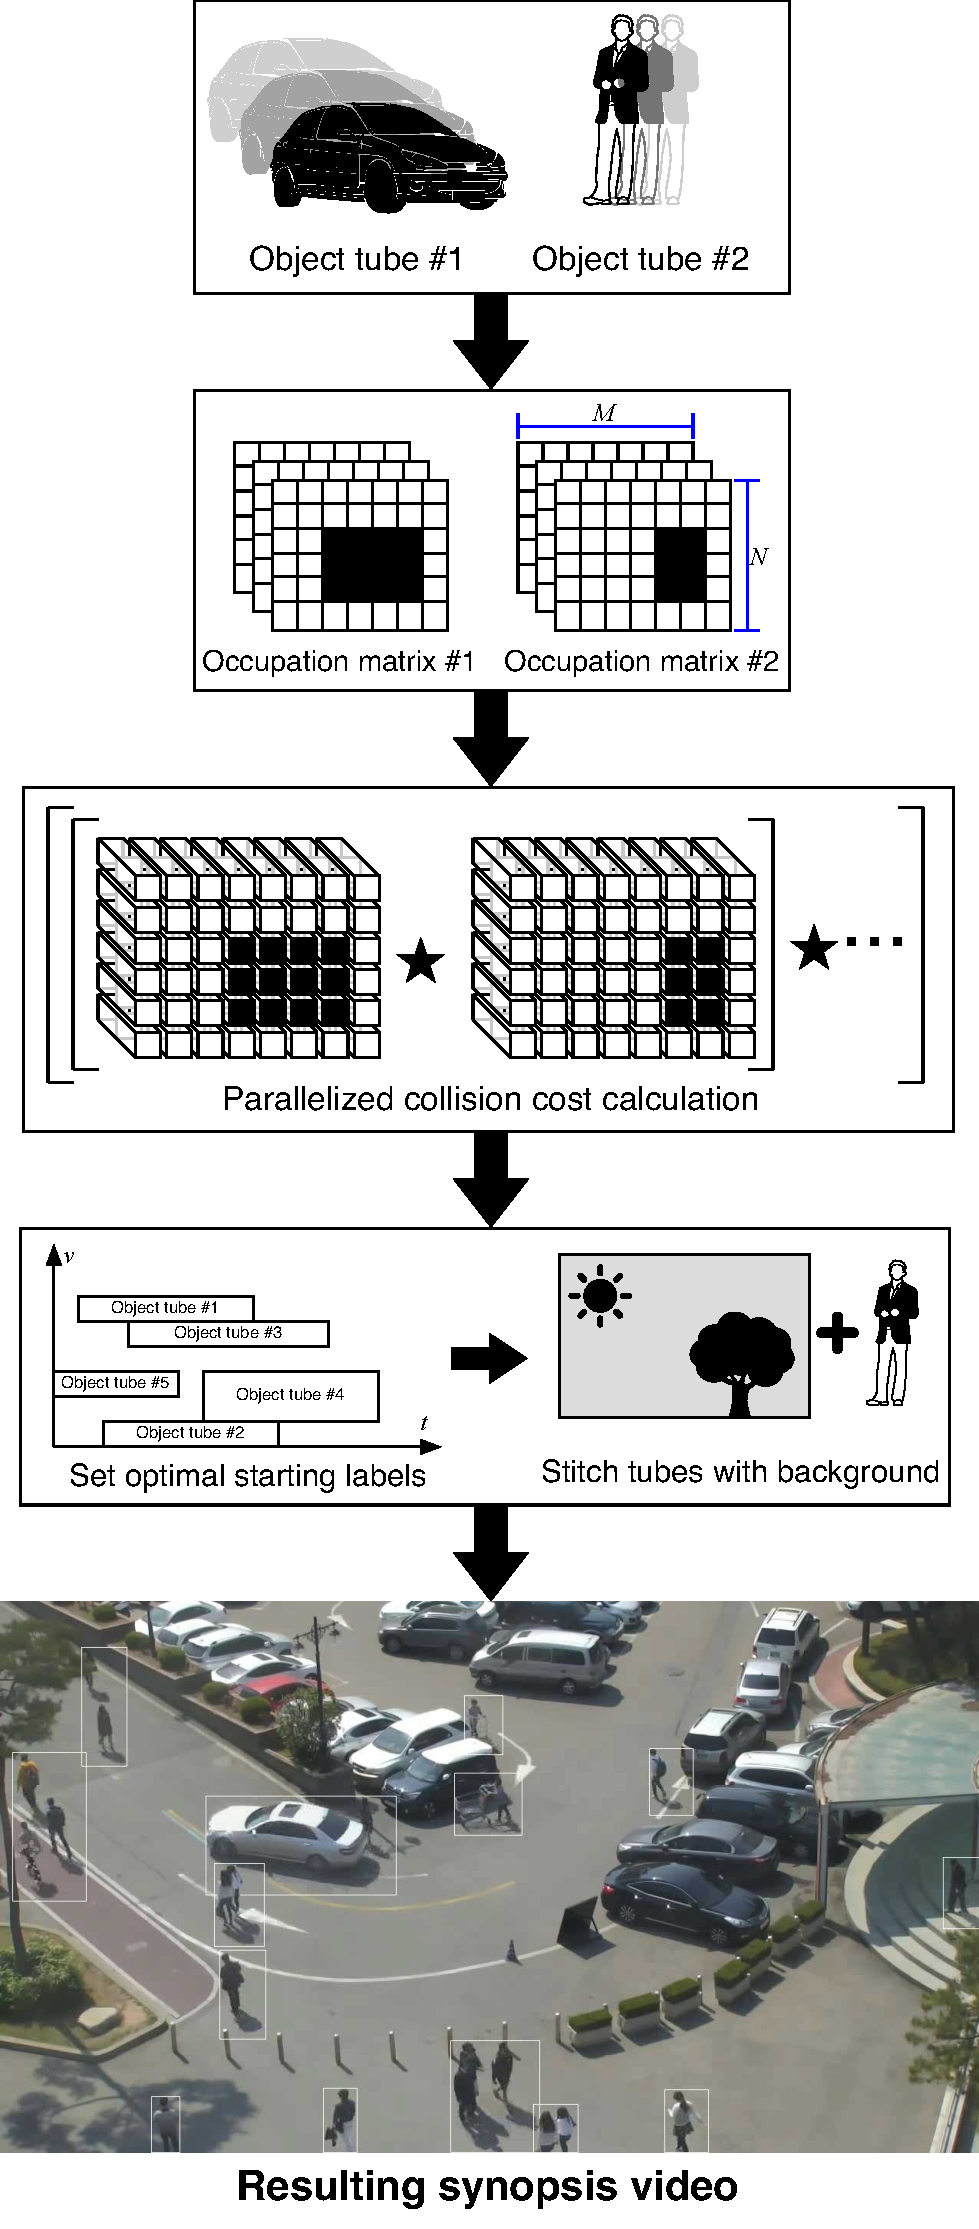
\includegraphics[width=\linewidth]{flowchart.pdf}
\caption{Flowchart of the proposed online video synopsis framework. At the beginning, foreground of the object tube is reshaped into the 3D occupation matrix. We use this matrix representation to calculate the collision energy fast in conjunction with parallel processing and Fourier transform. Afterwards, we determine optimal starting labels for tubes and stitch tubes with the background to generate a resulting synopsis video.}
\label{fig:flowchart}
\end{sidewaysfigure}

\section{Proposed tube rearrangement}
\label{sec:proposed}
In this section, the definition of $E_c$ is reformulated using the occupation matrix and an efficient tube rearrangement algorithm for optimizing the objective function is proposed. In addition, two types of the occupation matrix (binary and probabilistic) are introduced and their characteristics are explained in detail. A flowchart of the proposed online video synopsis framework including the tube rearrangement algorithm is illustrated in Fig.~\ref{fig:flowchart}.

\subsection{Occupation matrix generation}
\label{sec:proposed:occ}
Each element of the occupation matrix $\textbf{M}_i (u,v,t)$ is either from Boolean or continuous domain, and represents the probability of existence for $i^{\rm{th}}$ object tube at position $(u,v)$ and time $t$ of a video whose spatial resolution is $H \times W$. The $i^{\rm{th}}$ occupation matrix $\textbf{M}_i$ is then formed by stacking resized binary foreground masks of the object over multiple frames. The resized foreground mask has $M \times N$ resolution, where $M$ and $N$ have much smaller values than the width and height of the original video ($M \ll H$ and $N \ll W$). In this dissertation, two strategies of resizing will be introduced in following subsections and they determine the type of resulting occupation matrix: binary and probabilistic.

\subsubsection{Binary occupation matrix}
\label{sec:proposed:occ:binary}
The binary occupation matrix, $\textbf{M}^b$, does not allow gray area value to represent the existence of objects; it can only have 1s and 0s. Let assume that the foreground mask of the $i^{\rm{th}}$ object is denoted as $\textbf{F}_i(x,y,t) \in \mathbb{B}$; then, $\textbf{M}_i^b(u,v,t)$ is defined as
\begin{equation}
\label{eq:bin_occ}
\textbf{M}_i^b(u,v,t)=
\begin{cases}
1 & \sum_{(x,y) \in C(u,v)}\textbf{F}_i(x,y,t) \neq 0 \\
0 & \rm{otherwise},
\end{cases}
\end{equation}
where $C(u,v)$ is a set of 2D coordinates $(x,y)$. Based on (\ref{eq:bin_occ}), to calculate a single element of $\textbf{M}_i^b$, we need to examine the value of $\textbf{F}_i$ for every coordinate in $C(u,v)$. The definition of $C(u,v)$ is given by
\begin{equation}
C(u,v)=\left\{ (x,y) \mid x \in X(u), y \in Y(v) \right\},
\end{equation}
where $X(u)$ and $Y(v)$ are sets of $x$ and $y$ coordinates, respectively.
\begin{equation}
X(u)=\left\{ x \;\middle|\; \round*{\frac{W}{N}u} \leq x < \round*{\frac{W}{N}\left( u + 1 \right)} \right\},
\end{equation}
\begin{equation}
Y(v)=\left\{ y \;\middle|\; \round*{\frac{M}{H}v} \leq y < \round*{\frac{M}{H}\left( v + 1 \right)} \right\}.
\end{equation}

Due to the condition $\left( \sum_{(x,y) \in C(u,v)}\textbf{F}_i(x,y,t) \neq 0 \right)$ in (\ref{eq:bin_occ}), even a single pixel of $\textbf{F}_i(x,y,t)$ can produce a response in $\textbf{M}_i^b(u,v,t)$. Therefore, $\textbf{M}_i^b$ exaggerates the occupation region of the object tube in the video sequence. An example of the binary occupation matrix generation is depicted in Fig.~\ref{}.


\subsubsection{Probabilistic occupation matrix}
\label{sec:proposed:occ:prob}
Since the probabilistic occupation matrix, $\textbf{M}_i^p$, represents the existence of the object tube with continuous value, it can provide more precise information than $\textbf{M}_i^b$. Each element of $\textbf{M}_i^p$ is calculated as
\begin{equation}
\label{eq:prob_occ}
\textbf{M}_i^p(u,v,t)= \frac{\sum_{(x,y) \in C(u,v)}\textbf{F}_i(x,y,t)}{|C(u,v)|}.
\end{equation}

Based on (\ref{eq:prob_occ}), more 1 value of $\textbf{F}_i$ at coordinates in $C(u,v)$

\subsubsection{}
 Therefore, this representation provides coarse information about the object's positions in the video, and allows the calculation the collision energy between the object tubes efficiently. The type of the occupation matrix is determined 

\subsection{Objective function}
To generate more condensed and less complicated synopsis videos, collisions between object tubes as well as the length of the synopsis video are considered simultaneously during the tube rearrangement. Assume that the $i^\textrm{\tiny{th}}$ and $j^\textrm{\tiny{th}}$ object tubes have starting labels of $l_i$ and $l_j$ in the synopsis video. A collision energy between two objects $E_C (l_i,l_j)$ is defined as a sum of element-wise multiplications of $\textbf{M}_i$ and $\textbf{M}_j$.
\begin{equation}
\label{eq:collision_cost}
E_C(l_i,l_j) = \sum_{u=1}^{M}\sum_{v=1}^{N}\sum_{t=t_\textrm{\tiny{min}}}^{t_\textrm{\tiny{max}}} \textbf{M}_i(u,v,t)\textbf{M}_j(u,v,t),
\end{equation}
where $t_\textrm{\tiny{min}}$ and $t_\textrm{\tiny{max}}$ are minimum and maximum values of the overlapped temporal domain. Detailed calculations of $t_\textrm{\tiny{min}}$ and $t_\textrm{\tiny{max}}$ are
\begin{equation}
\label{eq:t_min}
t_\textrm{\tiny{min}} = \max(l_i, l_j),
\end{equation}
\begin{equation}
\label{eq:t_max}
t_\textrm{\tiny{max}} = \min(T_i + l_i, T_j + l_j),
\end{equation}
where $T_i$ and $T_j$ are frame lengths of the $i^\textrm{\tiny{th}}$ and $j^\textrm{\tiny{th}}$ object tubes, respectively.

A length energy $E_L (l_i,l_j)$ is defined as the frame length of the synopsis video when two object tubes have starting labels of $l_i$ and $l_j$.
\begin{equation}
\label{eq:length_cost}
E_L(l_i, l_j) = \max(T_i + l_i, T_j + l_j) - \min(l_i, l_j).
\end{equation}
An objective function $E(l_i,l_j)$ is calculated as a weighted sum of the collision and length energies.
\begin{equation}
\label{eq:obj_func}
E(l_i, l_j) = E_C(l_i, l_j) + \lambda E_L(l_i, l_j),
\end{equation}
where $\lambda$ is a weighting parameter adjusting the importance of the length energy. The larger $\lambda$ generates the shorter synopsis video.

\subsection{Optimizing objective function}
As in other online video synopsis algorithms, the proposed tube rearrangement algorithm adopts the stepwise optimization strategy; therefore, starting labels of the object tubes are determined one by one through iterations. At the $i^\textrm{\tiny{th}}$ iteration of the optimization, the starting label of $i^\textrm{\tiny{th}}$ object tube $l_i$ is determined as
\begin{equation}
\label{eq:starting_label}
l_i = \arg\min_l E(l, L_{i-1}) \textrm{ subject to } l_i \geq 0,
\end{equation}
where $L_{i-1} = \{ {l}_{1},...,{l}_{i-1} \}$ is a set of starting labels determined after $i-1$ iterations. A constraint to the optimization ${l}_{i} \geq 0$ is used to alleviate chronological disorder in the synopsis video. In other words, since a negative $l_i$ means that ${i}^\textrm{\tiny{th}}$ tube appear prior to the first tube in the synopsis video, preventing such case increases a chance to keep chronological order of the tubes. To minimize~(\ref{eq:starting_label}), an occupation matrix $\textbf{M}_{i-1}^{*}$ corresponding to a label set $L_{i-1}$ is required, where each element of $\textbf{M}_{i-1}^{*}$  satisfies the following equation.
\begin{equation}
\label{eq:occ_mat_update}
\textbf{M}_{i-1}^{*}(u, v, t) = \textbf{M}_{i-1}(u, v, t - l_{i-1}) + \textbf{M}_{i-2}^{*}(u, v, l_{i-2}^{*}),
\end{equation}
where $l_{i-2}^{*} = \min L_{i-2}$. For the initial condition of~(\ref{eq:occ_mat_update}), $\textbf{M}_{1}^{*} = \textbf{M}_{1}$ and $l_{1}^{*} = l_{1} = 0$ are used. As shown in~(\ref{eq:occ_mat_update}), $\textbf{M}_{i}^{*}$ can represent collisions of multiple object tubes (more than two) because $\textbf{M}_{i}^{*} \in \rm I\!R$. 

\begin{algorithm}[t]
\caption{Proposed tube rearrangement algorithm}
\label{alg:proposed}

\begin{algorithmic}
\REQUIRE $\textbf{M}_{i}, i = 1,...,N$
\ENSURE $L_{N} = \{ l_{1},...,l_{N} \}$

\STATE $\textbf{M}_{1}^{*} = \textbf{M}_{1}$, $l_{1}^{*} = l_{1} = 0$, $L_{1} = \{ l_{1} \}$

\FOR {$i = 2$ to $N$}
	\STATE Calculate $\textbf{M}_{i} \star \textbf{M}_{i-1}^{*}$ using FFT and parallel processing
	\STATE Find a local optimum starting label $l_{i}$ by using~(\ref{eq:starting_label})
	\iffalse
	\STATE $l_{i} = \arg\min_{l} E(l, L_{i-1})$ subject to $l_{i} \geq 0$
	\fi
	\STATE Calculate $\textbf{M}_{i}^{*}$ from $\textbf{M}_{i}$ and $\textbf{M}_{i-1}^{*}$ by using~(\ref{eq:occ_mat_update})
	\iffalse
	\STATE $\textbf{M}_{i}^{*}(u, v, t) = \textbf{M}_{i}(u, v, t-l_{i}) + \textbf{M}_{i-1}^{*}(u, v, t-l_{i-1}^{*})$
	\fi
	\STATE $L_{i} = L_{i-1} \cup l_{i}$
	\STATE $l_{i}^{*} = \min L_{i}$
\ENDFOR

\RETURN $L_{N}$
\end{algorithmic}

\end{algorithm}

\subsection{Parallelized collision cost calculation}
During the optimization, the collision energy computation becomes a bottleneck for performance because the collision energy needs to be evaluated for every possible $l$ value. To restrict a range of $l$ values, let us assume that two occupation matrices overlap by at least one frame in the temporal domain. Under this restriction,~(\ref{eq:collision_cost}) is simplified by adopting a cross-correlation of two occupation matrices in the temporal domain as
\begin{equation}
\label{eq:collision_cost_pp}
\begin{aligned}
E_C(l_i, l_j) = \sum_{u=1}^{M} \sum_{v=1}^{N} \textbf{M}_{i} \star \textbf{M}_{j}(u, v, l_i - l_j)\\
= \sum_{u=1}^{M} \sum_{v=1}^{N} \sum_{t=-\infty}^{\infty} \textbf{M}_{i}\textbf{M}_{j}(u, v, t + l_i - l_j)
\end{aligned}
\end{equation}

As shown in~(\ref{eq:collision_cost_pp}), cross-correlations in the temporal domain are independent to the spatial domain. Therefore, $M \times N$ cross-correlations can be concurrently computed using multi-cores or GPU environments. Also, cross-correlation itself can be calculated efficiently by the FFT~\cite{Oppenheim2009}. A detailed procedure of the proposed tube rearrangement algorithm is presented in Algorithm~\ref{alg:proposed}.

\begin{figure}
\centering
\subfloat[Parking lot square I]
{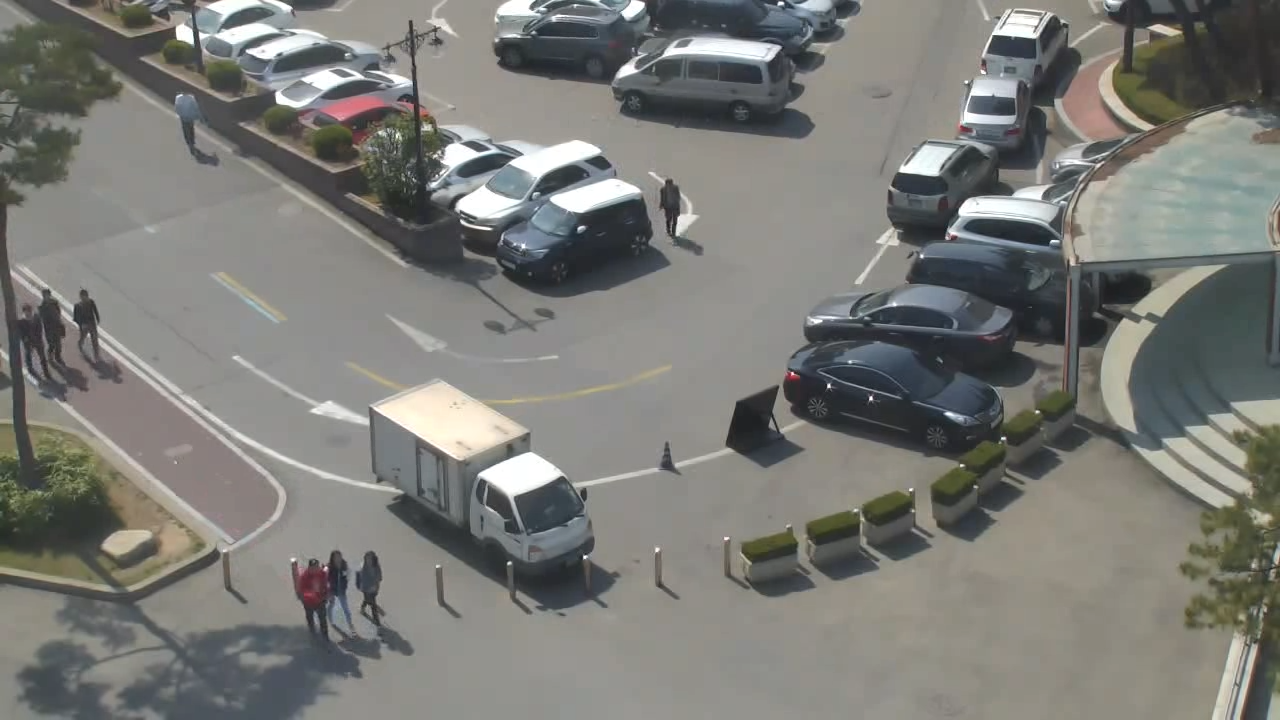
\includegraphics[width=0.45\linewidth]{fig/sidewalk.png}}
\label{fig:sidewalk}
\subfloat[Parking lot square II]
{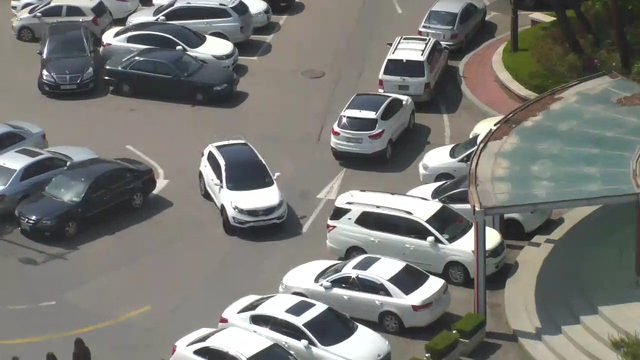
\includegraphics[width=0.45\linewidth]{fig/parking_lot.png}}
\label{fig:crossroadI}
\subfloat[Crossroad I]
{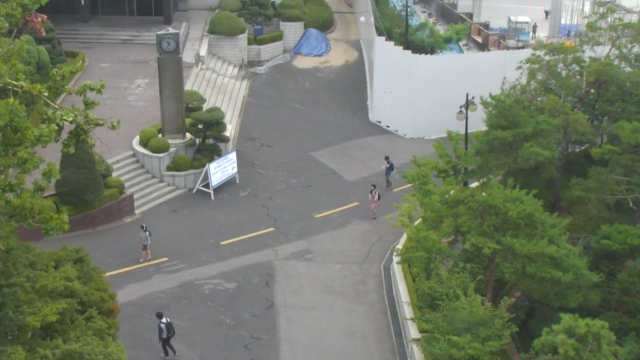
\includegraphics[width=0.45\linewidth]{fig/crossroad01.png}}
\label{fig:crossroadII}
\subfloat[Crossroad II]
{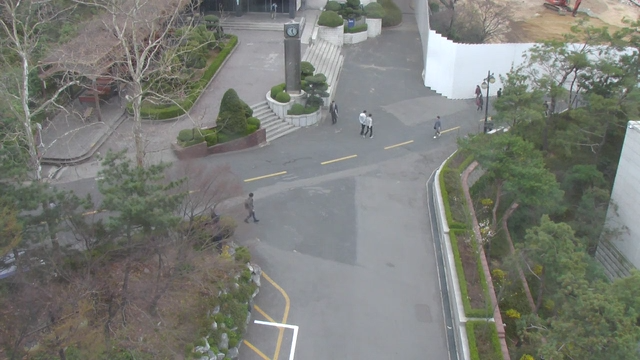
\includegraphics[width=0.45\linewidth]{fig/crossroad02.png}}
\label{fig:library}
\subfloat[Library lobby]
{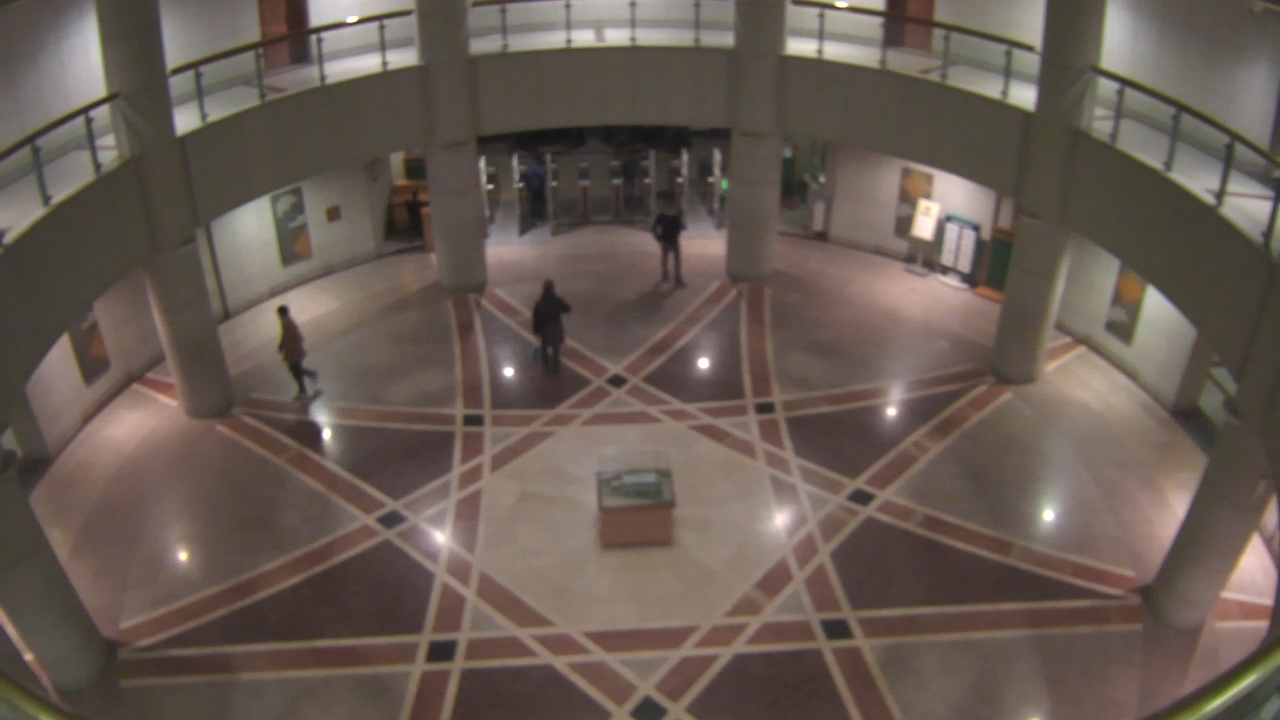
\includegraphics[width=0.45\linewidth]{fig/library.png}}
\label{fig:parking_lot}
\subfloat[Subway station plaza]
{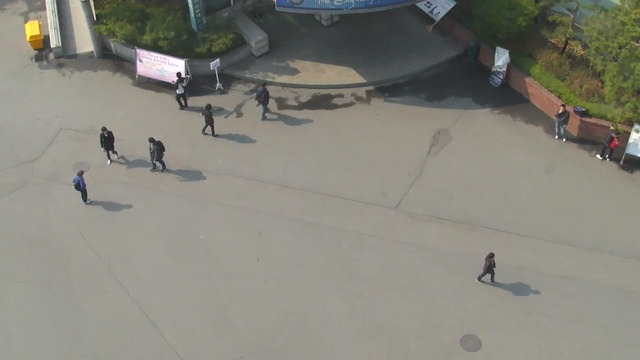
\includegraphics[width=0.45\linewidth]{fig/subway_entrance.png}}
\label{fig:subway_entrance}
\caption{Examples of the test sequences. All sequences were captured at Hanyang university, Seoul, Korea.}
\label{fig:examples}
\end{figure}

\begin{table}
\small
\begin{center}
\begin{tabular}{c|l|c|c|c|}
\cline{2-5}
 & Video Clips & Resolution & \# Frame & \# Tube\\
\hline
\multicolumn{1}{|c|}{1} & Parking lot square I & $1280 \times 720$ & 44,057 & 650\\
\hline
\multicolumn{1}{|c|}{5} & Parking lot square II & $640 \times 360$ & 107,946 & 271\\
\hline
\multicolumn{1}{|c|}{2} & Crossroad I & $640 \times 360$ & 85,766 & 291\\
\hline
\multicolumn{1}{|c|}{3} & Crossroad II & $640 \times 360$ & 106,459 & 937\\
\hline
\multicolumn{1}{|c|}{4} & Library lobby & $1280 \times 720$ & 49,679 & 316\\
\hline
\multicolumn{1}{|c|}{6} & Subway station plaza & $640 \times 360$ & 107,876 & 1038\\
\hline
\end{tabular}
\end{center}
\caption{List of test sequences used in the experiments}
\label{tb:video_list}
\end{table}

\section{Online video synopsis framework}
\label{sec:framework}
The proposed tube rearrangement algorithm is based on the online framework. Similar to existing online frameworks, the proposed framework consists of four stages: background modeling, object tube generation, tube rearrangement, and object stitching. 

During the background modeling stage, the foreground of the object is separated from the background by a well-known Gaussian mixture model~\cite{Zivkovic2004}. In the object tube generation stage, foregrounds that belong to the same object are associated by using the Hungarian algorithm~\cite{Kuhn1955} to generate the object tubes. Then, the generated object tubes are stored and maintained in a queue. When the size of the queue exceeds $K$, the starting labels of the object tubes in the queue are determined by the tube rearrangement algorithm, and the entire contents of the queue are cleared. After determining the starting labels, the corresponding object tubes are stitched back into the background to generate a small portion of the synopsis video. For a stitching algorithm, the Poisson image editing~\cite{Perez2003} is utilized. 

Because the aforementioned process generates the synopsis video in a stepwise fashion, a discontinuity of motion flow problem~\cite{Fu2014} occurs when merging small portions of the synopsis video into the complete one. This problem can be solved by considering the tails of the object tubes in the previous step during the current rearrangement step.

\section{Experimental Results}
\label{sec:exp}
In this section, the performance of the proposed tube rearrangement algorithm is evaluated by using four metrics: frame condensation ratio (FR), compact ratio (CR), overlap ratio (OR), and running time (RT). The experiments are conducted on a 4-core 4.0 GHz computer with 32 GB of memory. For the test sequences, six video clips are captured at four different places: a parking lot square, a crossroad, a library lobby, and a subway station plaza. Detail characteristics of the test sequences are summarized in Table~\ref{tb:video_list}. Some examples of the test sequences are depicted in Fig.~\ref{fig:examples}. The experiments are designed to 1) prove the efficiency of the parallelized tube rearrangement and 2) compare performances of several different online tube rearrangement algorithms.

\subsection{Efficiency of parallelized tube rearrangement}

To show the efficiency of our proposed parallelization scheme, parallelized and non-parallelized versions of the proposed algorithm are compared in terms of running time. A result of the comparison is illustrated in Fig.~\ref{fig:RT}. According to the results, the parallelized version is approximately 2.5 times faster than the non-parallelized version. Because the current parallelized version is based on CPU multi-threading, the proposed algorithm can be further efficiently computed with GPU-based parallelization.

\begin{figure}[t]
\begin{center}
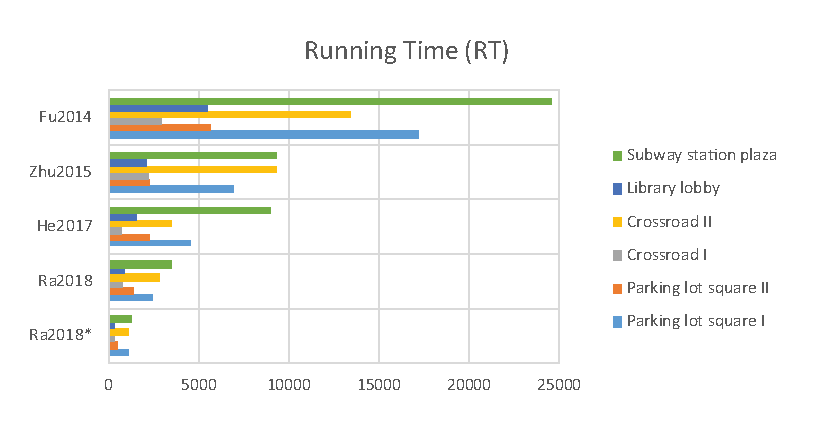
\includegraphics[width=0.9\linewidth]{RT.eps}
\end{center}
   \caption{Running times of the different tube rearrangement algorithms for six test sequences. An asterisk (*) indicates the parallelized version of the proposed algorithm.}
\label{fig:RT}
\end{figure}

\begin{figure}[t]
\begin{center}
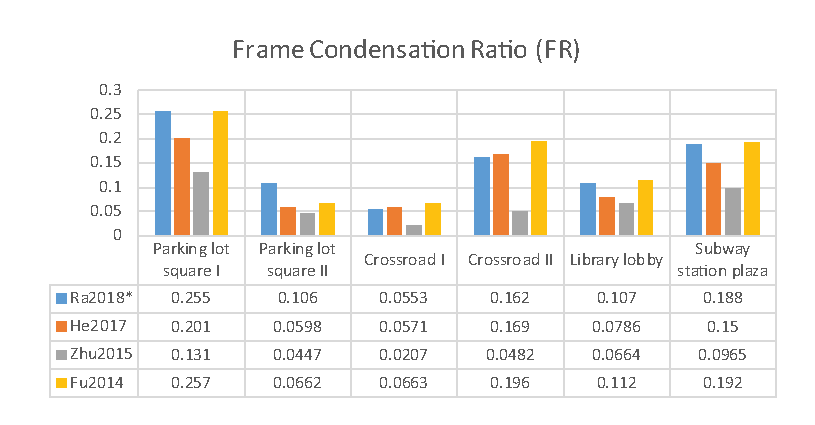
\includegraphics[width=0.9\linewidth]{FCR.eps}
\end{center}
   \caption{Frame condensation ratios of different tube rearrangement algorithms for six test sequences.}
\label{fig:FCR}
\end{figure}

\begin{figure}[t]
\begin{center}
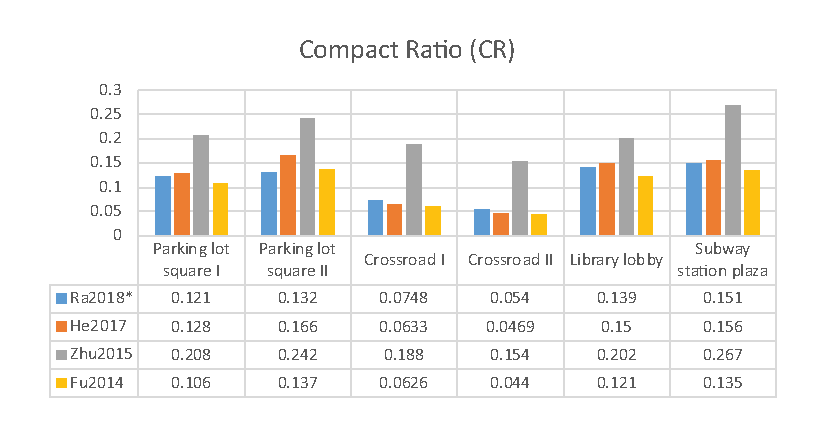
\includegraphics[width=0.9\linewidth]{CR.eps}
\end{center}
   \caption{Compact ratios of the different tube rearrangement algorithms for six test sequences.}
\label{fig:CR}
\end{figure}

\begin{figure}[t]
\begin{center}
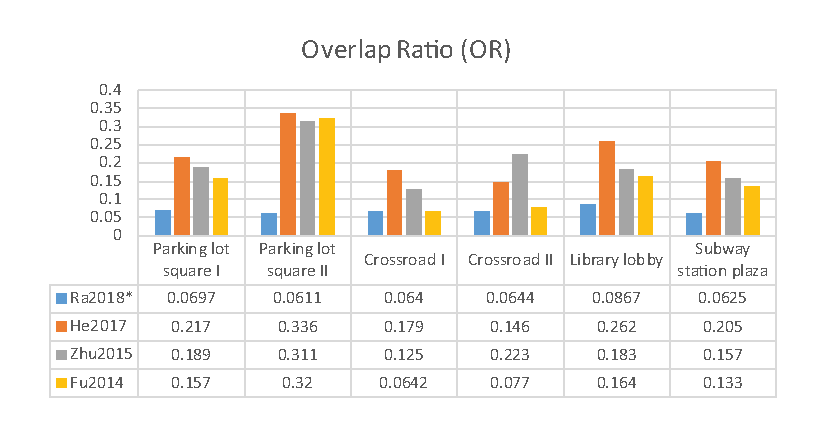
\includegraphics[width=0.9\linewidth]{OR.eps}
\end{center}
   \caption{Overlap ratios of the different tube rearrangement algorithms for six test sequences.}
\label{fig:OR}
\end{figure}

\subsection{Comparisons of different online tube rearrangement algorithms}
We have reproduced three recently introduced online tube rearrangement algorithms to compare and analyze the performance of the proposed algorithm. For fair comparisons, the required parameters of existing algorithms are set the same as in the original papers. Note that existing algorithms have not employed any spatial subsampling. Results of the comparisons are illustrated in~\cref{fig:RT,fig:FCR,fig:CR,fig:OR}. For FR, the proposed algorithm achieved the second-best performance in overall. For CR, the algorithm of Zhu~\etal~\cite{JianqingZhu2015} performed the best, while the others do not show significant differences. On the other hand, regarding RT and OR, the proposed algorithm outperformed other algorithms by a wide margin. Especially for RT, even a non-parallelized version has an advantage over existing algorithms. The experiments show that the proposed algorithm can efficiently handle occlusions far better than existing ones, even with a large number of objects.

\section{Conclusion}
\label{sec:conc}
This letter proposes the parallelized tube rearrangement algorithm for online video synopsis. For reducing the computational bottleneck caused by pairwise energy terms, the proposed algorithm concurrently computes the collision energy defined as multiplications of 3D occupation matrices by using an FFT. Throughout the experiments, the proposed algorithm outperformed existing algorithms in terms of computation time and overlap ratio, while its other performance metrics were comparable with those of other algorithms. Our future work will involve running the proposed algorithm on a GPU.

\bibliographystyle{IEEEtran}
\bibliography{IEEEabrv,video_synopsis}
\addcontentsline{toc}{section}{BIBLIOGRAPHY}

\end{document}

